% This is samplepaper.tex, a sample chapter demonstrating the
% LLNCS macro package for Springer Computer Science proceedings;
% Version 2.20 of 2017/10/04
%
\documentclass[runningheads]{llncs}
%
%\usepackage{graphicx}
% Used for displaying a sample figure. If possible, figure files should
% be included in EPS format.
%
% If you use the hyperref package, please uncomment the following line
% to display URLs in blue roman font according to Springer's eBook style:
% \renewcommand\UrlFont{\color{blue}\rmfamily}

%%%% Template Packages %%%%

%\usepackage[usenames]{color}
%\usepackage{xcolor}
%\usepackage{makeidx}
%\usepackage{graphicx}
%\usepackage{epsfig}
%\usepackage{xspace}
%\usepackage{pstricks}
%\usepackage{pst-node}
%\usepackage{pst-tree}
%\usepackage{pst-plot}
%\usepackage[nonumberlist, toc, style=super]{glossaries}
\usepackage[colorlinks]{hyperref}
%\usepackage{zed-csp}
%\usepackage{psfrag}
%\usepackage{ae}
%\usepackage{txfonts}
%\usepackage{ifthen}  
%\usepackage{alltt}
%\usepackage{url} 
%\usepackage{epsfig}
%\usepackage{listings}
%\usepackage{color,listings}
%\usepackage{rotating}
%\usepackage{longtable}
%\usepackage{fancyhdr}
%\usepackage[colorinlistoftodos]{todonotes}
%\usepackage{multirow}
%\usepackage{subfig}
%\usepackage{tabularx}
%\usepackage{array}
\usepackage[utf8]{inputenc}
%\usepackage{acronym}
\usepackage{setspace}

%\usepackage{titlesec}


%\usepackage{graphicx} % Required to insert images
%\usepackage{float}
%\usepackage{listings}

\usepackage{amsmath}
\usepackage{amsthm}
\usepackage{amssymb}

\usepackage{natbib}
\usepackage[nottoc,notlot,notlof]{tocbibind}

\usepackage{tikz}
\usetikzlibrary{backgrounds}
\usetikzlibrary{arrows}

\usepackage{algorithm}
\usepackage{algpseudocode}
\usepackage{algorithmicx}

\usepackage{subcaption}
%%%%%%%%%%%%%% GENERAL %%%%%%%%%%%%%%
\newcommand{\ct}{\sim}

\newcommand{\ms}[1]{\overset{#1}{\leftarrow}}
\newcommand{\mt}[1]{\overset{#1}{\rightarrow}}

%%%%%%%%%%%%%% GG %%%%%%%%%%%%%%
\newcommand{\neigh}[1]{\operatorname{neigh}_{#1}}
\newcommand{\isomorph}{\cong}
\newcommand{\scont}[2]{\eta_{#1}(#2)}
\newcommand{\cont}[2]{\operatorname{cont}_{#1}(#2)}
\newcommand{\emb}[1]{\operatorname{emb}(#1)}
\newcommand{\allgraphs}[1]{\mathcal{G}_{#1}}
\newcommand{\startG}[1]{Z_{#1}}
\newcommand{\pro}{\to}

%%%%%%%%%%%%%% TGG %%%%%%%%%%%%%%
\newcommand{\alltgraphs}[1]{\mathcal{TG}_{#1}}
\newcommand{\startTG}[1]{Z_{#1}}
\newcommand{\emptyTG}{\varepsilon}
\newcommand{\source}{\operatorname{s}}
\newcommand{\Source}{\operatorname{S}}
\newcommand{\target}{\operatorname{t}}
\newcommand{\Target}{\operatorname{T}}
\newcommand{\cderiv}[3]{
	\ifx\relax#2\relax%
	\overset{#1}{\Rrightarrow}_{#3}%
	\else
	\overset{#1,#2}{\Rrightarrow}_{#3}%
	\fi
}
\newcommand{\deriv}[3]{
	\ifx\relax#2\relax
	\overset{#1}{\Rightarrow}_{#3}
	\else
	\overset{#1,#2}{\Rightarrow}_{#3}
	\fi
}
\newcommand{\derivtr}[1]{
	\Rightarrow^*_{#1}
}
\newcommand{\tcderiv}[3]{
	\ifx\relax#2\relax
	\overset{#1}{\Rrightarrow}_{#3}
	\else
	\overset{#1,#2}{\Rrightarrow}_{#3}
	\fi
}
\newcommand{\tderiv}[3]{
	\ifx\relax#2\relax
	\overset{#1}{\Rightarrow}_{#3}
	\else
	\overset{#1,#2}{\Rightarrow}_{#3}
	\fi
}
\newcommand{\tderivtr}[1]{\Rightarrow^*_{#1}}

%%%% PAC %%%%
\newcommand{\cderivpac}[4]{\overset{#1,#2,#3}{\Rrightarrow}_{#4}}
\newcommand{\derivpac}[4]{
	\ifx\relax#3\relax
	\overset{#1,#2}{\Rightarrow}_{#4}
	\else
	\overset{#1,#2,#3}{\Rightarrow}_{#4}
	\fi}
\newcommand{\derivpacn}[2]{\Rightarrow^{#2}_{#1}}
\newcommand{\resolv}[1]{\overset{#1}{\rightarrowtail}}
\newcommand{\resolvn}[2]{\overset{#1}{\rightarrowtail}^{#2}}
\newcommand{\derivpactr}[1]{\Rightarrow^*_{#1}}
\newcommand{\resolvtr}[1]{\rightarrowtail^*}

\newcommand{\tcderivpac}[4]{\overset{#1,#2,#3}{\Rrightarrow}_{#4}}
\newcommand{\tderivpac}[4]{
	\ifx\relax#3\relax
	\overset{#1,#2}{\Rightarrow}_{#4}
	\else
	\overset{#1,#2,#3}{\Rightarrow}_{#4}
	\fi
}
\newcommand{\tderivpacn}[2]{\Rightarrow^{#2}_{#1}}
\newcommand{\tresolv}[1]{\overset{#1}{\rightarrowtail}}
\newcommand{\tresolvn}[2]{\overset{#1}{\rightarrowtail}^{#2}}
\newcommand{\tderivpactr}[1]{\Rightarrow^*_{#1}}
\newcommand{\tresolvtr}[1]{\rightarrowtail^*_{#1}}



%%%%%%%%%%%%%% TIKZ %%%%%%%%%%%%%%
\tikzstyle{grammar}=[shorten >= 1pt, ->, draw=black!50, framed, background rectangle/.style={draw, rounded corners}, font=\scriptsize ]
\tikzstyle{graph}=[shorten >= 1pt, ->, draw=black!50, font=\scriptsize]
\tikzstyle{rid} = [inner sep=3pt, align=left, anchor=east]
\tikzstyle{nont}=[rectangle, inner sep=3pt, draw, fill=white, minimum width=5pt]
\tikzstyle{t}=[circle, inner sep=1pt, draw, fill=white, minimum width=5pt]
\tikzstyle{pac}=[circle, inner sep=1pt, draw, dotted, fill=white, minimum width=5pt]
\tikzstyle{empty}=[font=\Large, fill=white]
\tikzstyle{g}=[inner sep=3pt, fill=white]
\tikzstyle{lhs}=[inner sep=1pt, fill=white]
\tikzstyle{w}=[circle, inner sep=1pt, below=8pt, draw, fill=white, font=\tiny]
\tikzstyle{uw}=[circle, inner sep=1pt, above=8pt, draw, fill=white, font=\tiny]
\tikzstyle{edge}=[->, thin, -latex]
\tikzstyle{pacedge}=[->, thin, -latex, dotted]
\tikzstyle{edgeLabel}=[midway, above]
\tikzstyle{vledgeLabel}=[midway, left]
\tikzstyle{vredgeLabel}=[midway, right]
\tikzstyle{vbedgeLabel}=[above=3pt]
\tikzstyle{wedge}=[-, thin]
\tikzstyle{biedge}=[-, thin]
\tikzstyle{pipe}=[-, thick]
\tikzstyle{morph}=[-, thin, dashed, -latex]

\newcommand{\ridX}{-0.3}
\newcommand{\ridY}{0.5}
\newcommand{\lhsX}{-0.3}
\newcommand{\pipeUY}{-0.5}
\newcommand{\pipeBY}{0.5}

%% Scheme %%
\tikzstyle{scheme}=[shorten >= 1pt, ->, draw=black!50, framed, background rectangle/.style={draw, rounded corners}, font=\scriptsize ]
\tikzstyle{object}=[rectangle, inner sep=3pt, draw, fill=white, minimum width=5pt]
\tikzstyle{metaobject}=[rectangle, inner sep=3pt, draw, dashed, fill=white, minimum width=5pt]
\tikzstyle{activity}=[rectangle, inner sep=3pt, draw, fill=white, minimum width=5pt, rounded corners]

\begin{document}
%
\title{Model Transformation with Triple Graph Grammars and Non-terminal Symbols}
%
\titlerunning{Model Transformation with TGG and Non-terminal Symbols}
% If the paper title is too long for the running head, you can set
% an abbreviated paper title here
%
\author{William {da Silva}\inst{1,2}$^{(\text{\Letter})}$ \and
Max {Bureck}\inst{1} \and
Ina {Schieferdecker}\inst{1,2} \and
Christian {Hein}\inst{1}}
%
\authorrunning{W. da Silva et al.}
% First names are abbreviated in the running head.
% If there are more than two authors, 'et al.' is used.
%
\institute{Fraunhofer Fokus, Berlin, Germany \\
\email{\{william.bombardelli.da.silva,max.bureck,ina.schieferdecker, christian.hein\}@fokus.fraunhofer.de}\and
Technische Universit\"{a}t Berlin, Berlin, Germany}
%
\maketitle              % typeset the header of the contribution
%
\begin{abstract}
This work proposes a new graph grammar formalism, that introduces non-terminal symbols to triple graph grammars (TGG) and shows how to apply it to solving the model transformation problem. Our proposed formalism seems to suit code generation from models well, outperforms the standard TGG in the grammar size in one evaluated case and is able to express one transformation that we could not express with TGG. We claim, that such advantages make a formal specification written in our formalism easier to validate and less error-prone, what befits safety-critical systems specially well.

\keywords{NCE Graph Grammars  \and Triple Graph Grammars \and Model Transformation \and Model-based Development.}
\end{abstract}
%
%
%
\section{Introduction}
Quality of service is a very common requirement for software projects, especially for safety-critical systems. A technique that aims to assure and enhance quality of software is the model-based development approach, which consists of the use of abstract models to specify aspects of the system under construction. The use of such models often allows for cheaper tests and verification as well as facilitates discussions about the system, for more abstract models tend to reduce the complexity of the actual object of interest. 

The construction of a system with model-based development commonly requires the creation of various models in different levels of abstraction, in which case we are interested in generating models automatically from other models. One example of such a situation is the transformation of a UML diagram into source-code or the compilation of source-code into machine-code. This problem is known as model transformation. For safety-critical systems, automatic model transformation is attractive, because transformers can be verified for correction carefully once and used many times, whereas manually or ad-hoc transformations have to be checked each time.

Several approaches to solving the model transformation problem have been proposed so far. Some of them consist of using the theory of graph grammars to formalize models and describe relations between them. One of which is the triple graph grammar (TGG) approach \cite{schurr1994specification}, which consists of building context-sensitive grammars of, so-called, triple graphs.

Triple graphs are composed of three graphs, the source and the target graphs, representing two models, and the correspondence graph that connects the source and the target through morphisms. A triple graph can be used to express the relationship between two graphs through the morphisms between their vertices. In this sense, a TGG describes a language of pairs of graphs whose vertices have a certain relationship. For the context of model transformation, in which one is interested in defining a translator from a source model to a target model, a TGG can be used to describe the set of all correctly translated source models and its correspondent target models, in form of a language of triple graphs.

Despite the various positive aspects of TGG, like a well-founded theory and a reasonable tool support \cite{anjorin201620}, they may sometimes get too big or too difficult to be constructed correctly. We judge, this downside stems from the absence of the concept of non-terminal symbols in the TGG formalism. This concept allows, in the theory of formal languages, for a very effective representation of abstract entities in string grammars.

So, motivated by this benefit, we present in this paper a novel formalism that redefines the standard triple graph grammars and introduces the notion of non-terminal symbols to create a context-free triple graph grammar formalism, that has in some cases a smaller size and with which we could describe one transformation that we could not with standard TGG.

Our approach consists of (1) mixing an already existent context-free graph grammar formalism, called NCE graph grammar from \cite{janssens1982graph}, with the standard TGG formalism from \cite{schurr1994specification}, to create the NCE TGG and (2) constructing a model transformer that interprets a NCE TGG to solve the model transformation problem.

The remainder of this paper is as follows, in Section \ref{sec:rw}, we present the research publications related to this topic, in Section \ref{sec:gg-tgg}, we give the main definitions necessary to build our approach, in Section \ref{sec:bncetgg}, we propose our modified version of TGG, the NCE TGG, in Section \ref{sec:modeltrans} we argue that our approach can be used for model transformation, in Section \ref{sec:eval} we evaluate our results and, finally, in Section \ref{sec:conclusion} we summarize and close our discussion.

\section{Related Works}
\label{sec:rw}
In this section, we offer a short literary review on the graph grammar and triple graph grammar approaches that are more relevant to our work. We focus, therefore, on the context-free node label replacement approach for graph grammars, although, there is a myriad of different alternatives to it, for example, the algebraic approach \cite{ehrig1999handbook}. We refer to context-free grammars, inspired by the use of such classification for string grammars, in a relaxed way without any compromise to any definition.

%We divide the node label replacement approaches into context-sensitive and context-free approaches, we refer to context-sensitive and context-free grammars, inspired by the use of such classification for string grammars, in a relaxed way without any compromise to any definition of context-freeness for graph grammars. The context-sensitive field includes the \textit{layered graph grammar}, whose semantics consists of the replacement of graphs by other graphs governed by morphisms \cite{rekers1997defining} and for which exponential-time bottom-up parsing algorithms have been proposed \cite{rekers1995graph,bottoni2000efficient,furst2011improving}. Another context-sensitive formalism is the \textit{reserved graph grammar}, that is based on the replacement of directed graphs by necessarily greater directed graphs governed by simple embedding rules \cite{zhang2001context} and for which exponential and polynomial-time bottom-up algorithms have been proposed in \cite{zeng2005rgg+,zou2017partial}.

In the node label replacement context-free formalisms stand out the \textit{node label controlled graph grammar} (NLC) and its successor \textit{graph grammar with neighborhood-controlled embedding} (NCE). NLC is based on the replacement of one vertex by a graph, governed by embedding rules written in terms of the vertex's label \cite{rozenberg1986boundary}. For various classes of these grammars, there exist polynomial-time top-down and bottom-up parsing algorithms \cite{flasinski1993parsing,flasinski2014characteristics,rozenberg1986boundary,wanke1991algorithms}. The recognition complexity and generation power of such grammars have also been analyzed \cite{flasinski1998power,kim2012structure}. NCE occurs in several formulations, including a context-sensitive one, but here we focus on the context-free formulation, where one vertex is replaced by a graph, and the embedding rules are written in terms of the vertex's neighbors \cite{janssens1982graph,skodinis1998neighborhood}. For some classes of these grammars, polynomial-time bottom-up parsing algorithms and automaton formalisms were proposed and analyzed \cite{kim2001efficient,brandenburg2005finite}. In special, one of these classes is the \textit{boundary graph grammar with neighborhood-controlled embedding} (BNCE), that is used in our approach for model transformation.

Regarding TGG \cite{schurr1994specification}, a 20 years review of the realm is put forward by Anjorin et al. \cite{anjorin201620}. In special, advances are made in the direction of expressiveness with the introduction of application conditions \cite{klar2010extended} and of modularization \cite{anjorin2014modularizing}. Furthermore, in the algebraic approach for graph grammars, we have found proposals that introduce inheritance \cite{bardohl2004integrating,hermann2008typed} and variables \cite{hoffmann2005graph} to the formalisms. Nevertheless, we do not know any approach that introduces non-terminal symbols to TGG with the purpose of gaining expressiveness or usability. In this sense, our proposal brings something new to the current state-of-the-art.

\section{Graph Grammars and Triple Graph Grammars}
\label{sec:gg-tgg}
In this section, we introduce important definitions that are used throughout this paper. First, we present definitions regarding graphs, taken mainly from \cite{rozenberg1986boundary}, second, we introduce the NCE graph grammar \cite{janssens1982graph,kim2001efficient} and then, we express our understanding of TGG, backed by \cite{schurr1994specification}.

\begin{definition}
	\label{def:graph}
	A directed labeled graph $G$ over the finite set of symbols $\Sigma$, $G = (V, E, \phi)$ consists of a finite set of vertices $V$, a set of labeled directed edges $E \subseteq V \times \Sigma \times V$ and a total vertex labeling function $\phi : V \to \Sigma$. 
\end{definition}

We refer to directed labeled graphs often referred simply as graphs. For a fixed graph $G$ we refer to its components as $V_G$, $E_G$ and $\phi_G$. Moreover, we define the special empty graph as $\emptyGraph := (\emptyset, \emptyset, \emptyset)$ and we denote the set of all graphs over $\Sigma$ by $\allgraphs{\Sigma}$. Two graphs $G$ and $H$ are disjoint if, and only if, $V_G \cap V_H = \emptyset$. If $\phi_G(v) = a$ we say $v$ is labeled by $a$. In special, we do not allow loops (vertices of the form $(v,l,v)$), but multi-edges with different labels are allowed.

Two vertices $v$ and $w$ are neighbors if, and only if, $(v,l,w) \in E_G$ or $(w,l,v) \in E_G$. In this case, we say $(v,l,w)$ and $(w,l,v)$ are adjacent edges to $v$ and to $w$.

\begin{definition}
	\label{def:morphism}
	A morphism of graphs $G$ and $H$ is a total mapping $m: V_G \to V_H$.
\end{definition}

\begin{definition}
	An isomorphism of directed labeled graphs $G$ and $H$ is a bijective mapping $m: V_G \to V_H$ that maintains the connections between vertices and their labels, that is, $(v,l,w) \in E_G$ if, and only if, $(m(v),l,m(w)) \in E_H$ and $\phi_G(v) = \phi_H(m(v))$.
\end{definition}

If there exists an isomorphism of $G$ and $H$, then $G$ and $H$ are said to be isomorphic and we denote the equivalence class of all graphs isomorphic to G by $[G]$. Notice that, contrary to isomorphisms, morphisms do not require bijectivity nor label or edge-preserving properties.

\begin{definition}
	\label{def:gg}
	A graph grammar with neighborhood-controlled embedding (NCE graph grammar) $GG = (\Sigma, \Delta \subseteq \Sigma, S \in \Sigma, P)$ consists of a finite set of symbols $\Sigma$ that is called alphabet, a subset of the alphabet $\Delta \subseteq \Sigma$ that holds the terminal symbols (we define the complementary set of non-terminal symbols as $\Gamma := \Sigma \setminus \Delta$), a special symbol of the alphabet $S \in \Sigma$, that is called start symbol, and a finite set of production rules $P$ of the form $(A \pro R, \omega)$ where $A \in \Gamma$ is called left-hand side, $R \in \allgraphs{\Sigma}$ is called right-hand side and $\omega : V_R \pto 2^{\Sigma \times \Sigma}$ is the partial embedding function from $R$'s vertices to pairs of edge and vertex labels.
\end{definition}

Notice that, in the original definition of NCE graph grammars \cite{janssens1982graph}, the left-hand side of the productions were allowed to contain any connected graph. Moreover, only undirected graphs without edge labels were allowed. So, strictly speaking, the definition above characterizes actually a 1-edNCE graph grammar, that contains only one element in the left-hand side and a directed edge-labeled graph in the right-hand side. Nevertheless, for simplicity, we use the denomination NCE graph grammar, or simply graph grammar, to refer to a 1-edNCE graph grammar along this paper. Moreover, vertices from the right-hand sides of rules labeled by non-terminal (terminal) symbols are said to be non-terminal (terminal) vertices. And finally, we define, for convenience, the start graph of $GG$ as $\startG{GG} := (\{v_s\},\emptyset,\{v_s \mapsto S\})$. 

%\begin{definition}
%	A boundary graph grammar with neighborhood-controlled embedding (BNCE graph grammar) $GG$ is such that non-terminal vertices of the right-hand sides of rules are not neighbors. That is, the NCE graph grammar $GG$ is boundary if, and only if, all its rules' right-hand sides are $\Gamma\text{-boundary}$ graphs.
%\end{definition}

In the following, we present our concrete syntax inspired by the well-known Backus-Naur form to denote NCE graph grammar rules. Let $GG = (\{A, B, a, b,$ $ c, l, m\},$ $\{a, b, c, l, m\}, A, \{p,q\})$ be a graph grammar with production rules $p = (A \pro G,\omega)$ and $q = (A \pro H,\zeta)$ where $G = (\{v_1, v_2, v_3\}, \{(v_1,l,v_2), (v_2,m,v_3)\},$ $\{v_1 \mapsto B, v_2 \mapsto b, v_3 \mapsto c \})$, and $H = (\{u_1\}, \emptyset, \{u_1 \mapsto a\})$, we denote $p$ and $q$ together as\\
\begin{equation*}
	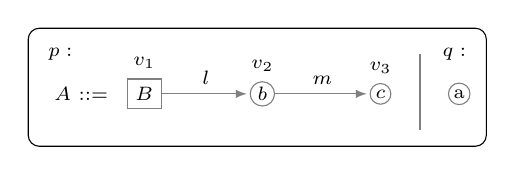
\begin{tikzpicture}[grammar]
	\node[rid] at (\ridX,\ridY) {$p:$};
	%The LHS
	\draw (\lhsX,0) node[lhs] (lhs) {$A$ ::=};
	
	%The RHS graph
	\draw (0.5,0) node[nont, label=90:$v_1$] (v1) {$B$};
	\draw (2,0) node[t, label=90:$v_2$] (v2) {$b$};
	\draw (3.5,0) node[t, label=90:$v_3$] (v3) {$c$};
	
	\draw[edge] (v1) -- (v2) node [edgeLabel] {$l$};
	\draw[edge] (v2) -- (v3) node [edgeLabel] {$m$};
	
	%The embedding
	%\draw node[w, label=0:$l;l;m$, label=-45:$a;b;c$] at (v1.south) (w-v1) {}
	%[wedge] (v1) -- (w-v1);
	
	%The next rule separator
	\draw[pipe] (4,\pipeBY) -- (4,\pipeUY);
	
	%The second RHS graph
	\node[rid] at (4.7,\ridY) {$q:$};
	\draw (4.5,0) node[t] (u1) {a};
	\end{tikzpicture}
\end{equation*}

Observe that, we use squares for non-terminal vertices, circles for terminal vertices, position the respective label inside the shape and the (possibly omitted) identifier over it. Near each edge is positioned its respective label. The embedding function is not included in the notation, so it is expressed separately, if necessary.

In the sequel, we introduce the dynamic aspects of NCE graph grammars by means of the concepts of derivation step, derivation, and language.

\begin{definition}
	\label{def:gg_dstep}
	Let $GG = (\Sigma, \Delta, S, P)$ be a NCE graph grammar and $G$ and $H$ be two graphs over $\Sigma$ that are disjoint to all right-hand sides from $P$, $G$ concretely derives in one step into $H$ with rule $r$ and vertex $v$, we write $G \cderiv{r}{v}{GG} H$ and call it a concrete derivation step, if, and only if, the following holds:
	\begin{align*}
		r & = (A \pro R, \omega) \in P \text{ and } A = \phi_G(v) \text{ and} \\
		V_H  & = (V_G \setminus \{v\}) \cup V_R \text{ and} \\
		E_H & = (E_G \setminus (\{(v,l,w) \st (v,l,w) \in E_G\} \cup \{(w,l,v) \st (w,l,v) \in E_G\})) \\
		& \cup E_R \\
		& \cup \{(w,l,t) \st (w,l,v) \in E_G \land (l,\phi_G(w)) \in \omega(t)\} \\
		& \cup \{(t,l,w) \st (v,l,w) \in E_G \land (l,\phi_G(w)) \in \omega(t)\} \text{ and} \\
		\phi_H & = (\phi_G \setminus \{(v,x) \st x \in \Sigma \}) \cup \phi_R
	\end{align*}
\end{definition}

Without loss of generality, we set $\omega(t) = \emptyset$ for all vertices $t$ without an image defined in $\omega$. Furthermore, let $H'$ be isomorphic to $H$, if $G$ \textit{concretely derives} in one step into $H$, we say $G$ \textit{derives} in one step into $H'$ and write $G \deriv{r}{v}{GG} H'$. 
	
When $GG$, $r$ or $v$ are clear in the context or irrelevant we might omit them and simply write $G \cderiv{}{}{} H$ or $G \deriv{}{}{} H$. Moreover, we denote the reflexive transitive closure of $\deriv{}{}{}$ by $\derivtr{}$ and, for $G \derivtr{} H'$, we say $G$ derives into $H'$.

A concrete derivation can be informally understood as the replacement of a non-terminal vertex $v$ and all its adjacent edges in $G$ by a graph $R$ plus edges $e$ between former neighbors $w$ of $v$ and some vertices $t$ of $R$, provided $e$'s label and $w$'s label are in the embedding specification $\omega(t)$. That is, the embedding function $\omega$ of a rule specifies which neighbors of $v$ are to be connected with which vertices of $R$, according to their labels and the adjacent edges' labels. The process that governs the creation of these edges is called embedding and can occur in various forms in different graph grammar formalisms. We opted for a rather simple approach, in which the edges' directions and labels are maintained.

\begin{definition}
	A derivation $D$ in the grammar $GG$ is a non-empty sequence of derivation steps and is written as
	\begin{equation*}
		D = (G_0 \deriv{r_0}{v_0}{} G_1 \deriv{r_1}{v_1}{} G_2 \deriv{r_2}{v_2}{} \dots \deriv{r_{n-1}}{v_{n-1}}{} G_n)
	\end{equation*}
\end{definition}

\begin{definition}
	\label{def:language}
	The language $L(GG)$ generated by the grammar $GG$ is the set of all graphs containing only terminal vertices derived from the start graph $\startG{GG}$, that is
	\begin{equation*}
		L(GG) = \{H \text{ is a graph over } \Delta \text{ and } \startG{GG} \derivtr{} H\}
	\end{equation*}
\end{definition}

Below, we give one example of a grammar whose language consists of all chains of one or more vertices with interleaved vertices labeled with $a$ and $b$.

%Examples (chains)
\begin{example}{}
	$GG = (\{S,A,B,a,b,c\}, \{a,b,c\}, S, P)$, where $P = \{r_0, r_1, r_2, r_3, r_4, $ $r_5\}$ is denoted by
	
		\noindent
	\begin{minipage}[t]{.27\textwidth}
		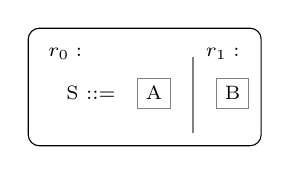
\begin{tikzpicture}[grammar]
		\node[rid] at (\ridX,\ridY) {$r_0:$};
		%The LHS
		\draw (\lhsX,0) node[lhs] (lhs) {S ::=};
		
		%The RHS graph
		\draw (0.5,0) node[nont] (v1) {A};
		
		%The next rule separator
		\draw[pipe] (1,-0.5) -- (1,\ridY);
		
		%The second RHS graph
		\node[rid] at (1.7,\ridY) {$r_1:$};
		\draw (1.5,0) node[nont] (v2) {B};
		\end{tikzpicture}
	\end{minipage}%
	\begin{minipage}[t]{.37\textwidth}
		\begin{tikzpicture}[grammar]
		\node[rid] at (\ridX,\ridY) {$r_2:$};
		%The LHS
		\draw (\lhsX,0) node[lhs] (lhs) {A ::=};
		
		%The RHS graph
		\draw (0.5,0) node[t] (v3) {a};
		\draw (1.5,0) node[nont] (v4) {B};
		
		\draw[edge] (v3) -- (v4) node [edgeLabel] {$c$};
		
		\draw node[w, label=0:$c$, label=-45:$b$] at (v3.south) (w-v3) {}
		[wedge] (v1) -- (w-v3);
		
		%The next rule separator
		\draw[pipe] (2,\pipeBY) -- (2,\pipeUY);
		
		%The second RHS graph
		\node[rid] at (2.7,\ridY) {$r_3:$};
		\draw (2.5,0) node[t] (v5) {a};
		\draw node[w, label=0:$c$, label=-45:$b$] at (v5.south) (w-v5) {}
		[wedge] (v5) -- (w-v5);
		\end{tikzpicture}
	\end{minipage}%
	\begin{minipage}[t]{.37\textwidth}
		\begin{tikzpicture}[grammar]
		\node[rid] at (\ridX,\ridY) {$r_4:$};
		%The LHS
		\draw (\lhsX,0) node[lhs] (lhs) {B ::=};
		
		%The RHS graph
		\draw (0.5,0) node[t] (v6) {b};
		\draw (1.5,0) node[nont] (v7) {A};
		
		\draw[edge] (v3) -- (v4) node [edgeLabel] {$c$};
		
		\draw node[w, label=0:$c$, label=-45:$a$] at (v6.south) (w-v6) {}
		[wedge] (v1) -- (w-v6);
		
		%The next rule separator
		\draw[pipe] (2,\pipeBY) -- (2,\pipeUY);
		
		%The second RHS graph
		\node[rid] at (2.7,\ridY) {$r_5:$};
		\draw (2.5,0) node[t] (v8) {b};
		\draw node[w, label=0:$c$, label=-45:$a$] at (v8.south) (w-v8) {}
		[wedge] (v8) -- (w-v8);
		\end{tikzpicture}
	\end{minipage}
	with $\omega_0 = \omega_1 = \emptyset$, $\omega_2(u_{21}) = \omega_3(u_{31}) = \{(c,b)\}$ and $\omega_4(u_{41}) = \omega_5(u_{51}) = \{(c,a)\}$ being the complete definition of the embedding functions of the rules, $r_0, r_1, r_2, r_3, r_4, r_5$ respectively.
	
	The graph $G=$
	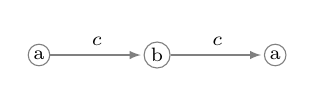
\begin{tikzpicture}[graph]
	\draw (0,0) node[t] (v1) {a};
	\draw (1.5,0) node[t] (v2) {b};
	\draw (3,0) node[t] (v3) {a};
	\draw[edge] (v1) -- (v2) node [edgeLabel] {$c$};
	\draw[edge] (v2) -- (v3) node [edgeLabel] {$c$};
	\end{tikzpicture}
	belongs to $L(GG)$ because it contains only terminal vertices and $\startG{GG}$ derives into it using the following derivation:
	\begin{equation*}
		\startG{GG} \deriv{r_0}{v_0}{} 
		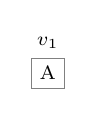
\begin{tikzpicture}[graph]
		\draw (0,0) node[nont, label=90:$v_1$] (v1) {A};
		\end{tikzpicture}
		\deriv{r_2}{v_1}{} 
		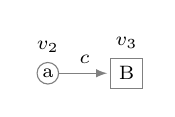
\begin{tikzpicture}[graph]
		\draw (1,0) node[t, label=90:$v_2$] (v2) {a};
		\draw (2,0) node[nont, label=90:$v_3$] (v3) {B};
		\draw[edge] (v2) -- (v3) node [edgeLabel] {$c$};
		\end{tikzpicture}
		\deriv{r_4}{v_3}{}
		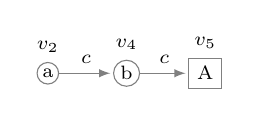
\begin{tikzpicture}[graph]
		\draw (1,0) node[t, label=90:$v_2$] (v2) {a};
		\draw (2,0) node[t, label=90:$v_4$] (v4) {b};
		\draw (3,0) node[nont, label=90:$v_5$] (v5) {A};
		\draw[edge] (v2) -- (v4) node [edgeLabel] {$c$};
		\draw[edge] (v4) -- (v5) node [edgeLabel] {$c$};
		\end{tikzpicture}
		\deriv{r_3}{v_5}{}
		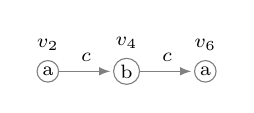
\begin{tikzpicture}[graph]
		\draw (0,0) node[t, label=90:$v_2$] (v2) {a};
		\draw (1,0) node[t, label=90:$v_4$] (v4) {b};
		\draw (2,0) node[t, label=90:$v_6$] (v6) {a};
		\draw[edge] (v2) -- (v4) node [edgeLabel] {$c$};
		\draw[edge] (v4) -- (v6) node [edgeLabel] {$c$};
		\end{tikzpicture}
	\end{equation*}
\end{example}

Building upon the concepts of graphs and graph grammars, we present, in the following, our understanding over triple graphs and triple graph grammars, supported by the TGG specification from \cite{schurr1994specification}.

\begin{definition}
	A directed labeled triple graph $TG = G_s \ms{m_s} G_c \mt{m_t} G_t$ over $\Sigma$ consists of three disjoint directed labeled graphs over $\Sigma$ (see Definition \ref{def:graph}), respectively, the source graph $G_s$, the correspondence graph $G_c$ and the target graph $G_t$, together with two injective morphisms (see Definition \ref{def:morphism}) $m_s: V_{G_c} \to V_{G_s}$ and $m_t : V_{G_c} \to G_{G_t}$.
\end{definition}

We refer to directed labeled triple graphs are often simply as triple graphs in this paper and we might omit the morphisms' names in the notation. We also advise that in the literature, triple graphs are often modeled as typed graphs, but we judge that for our circumstance labeled graphs fit better and we are convinced that such divergence does not threaten the validity of our approach.

%\begin{definition}
%	A $\Gamma\text{-boundary}$ triple graph $TG = G_s \ms{} G_c \mt{} G_t$ is such that $G_s$, $G_c$ and $G_t$ are $\Gamma\text{-boundary}$ graphs.
%\end{definition}

Below, we introduce the standard definition of TGG.

\begin{definition}
	\label{def:stgg}
	A triple graph grammar $TGG = (\Sigma, \Delta \subseteq \Sigma, S \in \Sigma, P)$ consists of, analogously to graph grammars (see Definition \ref{def:gg}), an alphabet $\Sigma$, a set of terminal symbols $\Delta$, a start symbol $S$ and a set of production rules $P$ of the form $L \pro R$ with $L = L_s \ms{} L_c \mt{} L_t$ and $R = R_s \ms{} R_c \mt{} R_t$ and $L \subseteq R$.
\end{definition}

As the reader should notice, this definition of TGG does not fit our needs optimally, because it defines a context-sensitive graph grammar, whereas we wish a context-free graph grammar to use together with the NCE graph grammar formalism. Hence, we refine it, in the next section, to create a NCE TGG, that fits our context better.

\section{NCE TGG: A TGG with Non-terminal Symbols}
\label{sec:bncetgg}
In this section, we put forward our first contribution, that is the result of mixing the NCE and the TGG grammars.

\begin{definition}
	A triple graph grammar with neighborhood-controlled embedding (NCE TGG) $TGG = (\Sigma, \Delta \subseteq \Sigma, S \in \Sigma, P)$ consists of an alphabet $\Sigma$, a set of terminal symbols $\Delta$ (also define $\Gamma := \Sigma \setminus \Delta$), a start symbol $S$ and a set of production rules $P$ of the form $(A \pro (R_s \ms{} R_c \mt{} R_t), \omega_s, \omega_t)$ with $A \in \Gamma$ being the left-hand side, $(R_s \ms{} R_c \mt{} R_t) \in \alltgraphs{\Sigma}$ the right-hand side and $\omega_s : V_{R_s} \pto 2^{\Sigma \times \Sigma}$ and $\omega_t : V_{R_t} \pto 2^{\Sigma \times \Sigma}$ the partial embedding functions from the right-hand side's vertices to pairs of edge and vertex labels.
\end{definition}

For convenience, define also the start triple graph of $TGG$ as $\startTG{TGG} := Z_s \ms{ms} Z_c \mt{mt} Z_t$ where $Z_s = (\{s_0\},\emptyset,\{s_0 \mapsto S\})$, $Z_c = (\{c_0\},\emptyset,\{c_0 \mapsto S\})$, $Z_t = (\{t_0\},\emptyset,\{t_0 \mapsto S\})$, $ms = \{c_0 \mapsto s_0 \}$ and $mt = \{c_0 \mapsto t_0 \}$.

The most important difference between the traditional TGG and the NCE TGG is that the former allows any triple graph to occur in the left-hand sides, whereas the latter only one symbol. In addition to that, traditional TGG requires that the whole left-hand side occur also in the right-hand side, that is to say, the rules are monotonic. Therewith, embedding is not an issue, because an occurrence of the left-hand side is not effectively replaced by the right-hand side, instead, only new vertices are added. On the other hand, NCE TGG has to deal with embedding through the embedding function.

In the following, the semantics for NCE TGG is presented analogously to the semantics for NCE graph grammars.

\begin{definition}
	\label{def:tgg_dstep}
	Let $TGG = (\Sigma, \Delta, S, P)$ be a NCE TGG and $G = G_s \ms{g_s} G_c \mt{g_t} G_t$ and $H = H_s \ms{h_s} H_c \mt{h_t} H_t$ be two triple graphs over $\Sigma$ that are disjoint to all right-hand sides from $P$, $G$ concretely derives in one step into $H$ with rule $r$ and distinct vertices $v_s, v_c, v_t$, we write $G \tcderiv{r}{v_s,v_c,v_t}{TGG} H$ if, and only if, the following holds:
	\begin{align*}
		r & = (A \pro (R_s \ms{r_s} R_c \mt{r_t} R_t), \omega_s, \omega_t) \in P \text{ and } \\
		A & = \phi_{G_s}(v_s) = \phi_{G_c}(v_c) = \phi_{G_t}(v_t) \text{ and}\\
		V_{H_s}  & = (V_{G_s} \setminus \{v_s\}) \cup V_{R_s} \text{ and}\\
		V_{H_c}  & = (V_{G_c} \setminus \{v_c\}) \cup V_{R_c} \text{ and}\\
		V_{H_t}  & = (V_{G_t} \setminus \{v_t\}) \cup V_{R_t} \text{ and}\\
		E_{H_s} & = (E_{G_s} \setminus (\{(v_s,l,w) \st (v_s,l,w) \in E_{G_s}\} \cup \{(w,l,v_s) \st (w,l,v_s) \in E_{G_s}\})) \\
		& \cup E_{R_s} \\
		& \cup \{(w,l,t) \st (w,l,v_s) \in E_{G_s} \land (l,\phi_{G_s}(w)) \in \omega_{s}(t)\} \\
		& \cup \{(t,l,w) \st (v_s,l,w) \in E_{G_s} \land (l,\phi_{G_s}(w)) \in \omega_{s}(t)\} \text{ and} \\
		E_{H_c} & = (E_{G_c} \setminus (\{(v_c,l,w) \st (v_c,l,w) \in E_{G_c}\} \cup \{(w,l,v_c) \st (w,l,v_c) \in E_{G_c}\})) \\
		& \cup E_{R_c} \text{ and} \\
		E_{H_t} & = (E_{G_t} \setminus (\{(v_t,l,w) \st (v_t,l,w) \in E_{G_t}\} \cup \{(w,l,v_t) \st (w,l,v_t) \in E_{G_t}\})) \\
		& \cup E_{R_t} \\
		& \cup \{(w,l,t) \st (w,l,v_t) \in E_{G_t} \land (l,\phi_{G_t}(w)) \in \omega_{t}(t)\} \\
		& \cup \{(t,l,w) \st (v_t,l,w) \in E_{G_t} \land (l,\phi_{G_t}(w)) \in \omega_{t}(t)\} \text{ and} \\
		h_s		& = (g_s \setminus \{(v_c,x) \st x \in V_{G_s}\}) \cup r_s  \\
		h_t		& = (g_t \setminus \{(v_c,x) \st x \in V_{G_t}\}) \cup r_t  \\
		\phi_{H_s} & = (\phi_{G_s} \setminus \{(v_s,x) \st x \in \Sigma\}) \cup \phi_{R_s} \text{ and}\\
		\phi_{H_c} & = (\phi_{G_c} \setminus \{(v_c,x) \st x \in \Sigma\}) \cup \phi_{R_c} \text{ and}\\
		\phi_{H_t} & = (\phi_{G_t} \setminus \{(v_t,x) \st x \in \Sigma\}) \cup \phi_{R_t}\\
	\end{align*}
\end{definition}

Without loss of generality, we set $\omega(t) = \emptyset$ for all vertices $t$ without an image defined in $\omega$. And, analogously to graph grammars, if $G \cderiv{r}{v_s,v_c,v_t}{TGG} H$ and $H' \in [H]$, then $G \tderiv{r}{v_s,v_c,v_t}{TGG} H'$, moreover the reflexive transitive closure of $\tderiv{}{}{}$ is denoted by $\tderivtr{}$ and we call these relations by the same names as before, namely, derivation in one step and derivation. We might also omit identifiers.

A concrete derivation of a triple graph $G = G_s \ms{g_s} G_c \mt{g_t} G_t$ can be informally understood as concrete derivations (see Definition \ref{def:gg_dstep}) of $G_s$, $G_c$ and $G_t$ according to the right-hand sides $R_s$, $R_c$ and $R_t$. The only remark is the absence of an embedding mechanism for the correspondence graph, whose edges are not important for our approach. Nevertheless, the addition of such a mechanism for the correspondence graph should not be a problem if it is desired.

\begin{definition}
	A derivation $D$ in the triple graph grammar $TGG$ is a non-empty sequence of derivation steps
	\begin{equation*}
		D = (G_0 \tderiv{r_0}{s_0,c_0,t_0}{} G_1 \tderiv{r_1}{s_1,c_1,t_1}{} G_2 \tderiv{r_2}{s_2,c_2,t_2}{} \dots \tderiv{r_{n-1}}{s_{n-1},c_{n-1},t_{n-1}}{} G_n)
	\end{equation*}
\end{definition}

\begin{definition}
	\label{def:tlanguage}
	The language $L(TGG)$ generated by the triple grammar $TGG$ is the set of all triple graphs containing only terminal vertices derived from the start triple graph $\startTG{TGG}$, that is
	\begin{equation*}
		L(TGG) = \{H \text{ is a triple graph over } \Delta \text{ and } \startTG{TGG} \tderivtr{} H\}
	\end{equation*}
\end{definition}

Our concrete syntax for NCE TGG is similar to the one for NCE graph grammars and is presented below by means of the Example \ref{ex:pseudocode2controlflow}. The only difference is at the right-hand sides, that include the morphisms between the correspondence graphs and source and target graphs depicted with dashed lines.

%Concrete syntax and examples (Pseudocode 2 Control Flow [sourcecode2controlflow])
\begin{example}
	\label{ex:pseudocode2controlflow}
	This example illustrates the definition of a NCE TGG that characterizes the language of all $Pseudocode$ graphs together with their respective $Controlflow$ graphs. A $Pseudocode$ graph is an abstract representation of a program written in a pseudo-code where vertices refer to \textit{actions}, \textit{ifs} or \textit{whiles} and edges connect these items together according to how they appear in the program. A $Controlflow$ graph is a more abstract representation of a program, where vertices can only be either a \textit{command} or a \textit{branch}.
	
	Consider, for instance, the program $main$, written in a pseudo-code, and the triple graph $TG$ in Figure \ref{fig:p2c-tg}. The triple graph $TG$ consists of the $Pseudocode$ graph of $main$ connected to the $Controlflow$ graph of the same program through the correspondence graph in the middle of them. In such graph, the vertex labels of the $Pseudocode$ graph $p, i, a, w$ correspond to the concepts of \textit{program}, \textit{if}, \textit{action} and \textit{while}, respectively. The edge label $f$ is given to the edge from the vertex $p$ to the program's first statement, $x$ stands for \textit{next} and indicates that a statement is followed by another statement, $p$ and $n$ stand for \textit{positive} and \textit{negative} and indicate which assignments correspond to the positive of negative case of the \textit{if}'s evaluation, finally $l$ stands for \textit{last} and indicates the last action of a loop. In the $Controlflow$ graph, the vertex labels $g, b, c$ stand for the concepts of \textit{graph}, \textit{branch} and \textit{command}, respectively. The edge label $r$ is given to the edge from the vertex $g$ to the first program's statement, $x, p$ and $n$ mean, analogous to the former graph, \textit{next}, \textit{positive} and \textit{negative}. In the correspondence graph, the labels $pg, ib, ac, wb$ serve to indicate which labels in the source and target graphs are being connected through the triple graph's morphism.
	%TODO: advise that command are not stuffed with further information that actually characterizes them. But it could be done with a future work on attributed graphs
	
	The main difference between the two graphs is the absence of the $w$ label in the $Controlflow$ graph, what makes it encode loops through the combination of $b$-labeled vertices and $x$-labeled edges.
	
	\begin{minipage}[h]{.48\textwidth}
	\begin{algorithmic}[!ht]
		\State \Program $main(n)$
		\If {$n < 0$}
			\State \Return $\Nothing$
		\Else
			\State $f \gets 1$ 
			\While {$n > 0$}
				\State $f \gets f * n$
				\State $n \gets n - 1$
			\EndWhile
			\State \Return $\Just f$
		\EndIf
	\end{algorithmic}
\end{minipage}
\begin{minipage}[h]{.5\textwidth}
	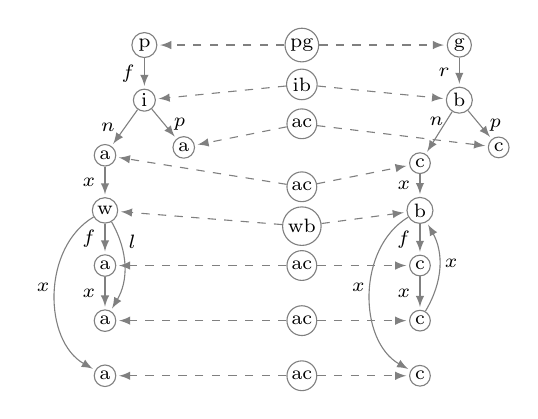
\begin{tikzpicture}[graph]
	\draw (1,0) node[t] (s1) {p};
	\draw (1,-0.7) node[t] (s2) {i};
	\draw (1.5,-1.3) node[t] (s3) {a};
	\draw (0.5,-1.4) node[t] (s4) {a};
	\draw (0.5,-2.1) node[t] (s5) {w};
	\draw (0.5,-2.8) node[t] (s6) {a};
	\draw (0.5,-3.5) node[t] (s7) {a};
	\draw (0.5,-4.2) node[t] (s8) {a};
	
	\draw[edge] (s1) -- (s2) node [vledgeLabel] {$f$};
	\draw[edge] (s2) -- (s3) node [vredgeLabel] {$p$};
	\draw[edge] (s2) -- (s4) node [vledgeLabel] {$n$};
	\draw[edge] (s4) -- (s5) node [vledgeLabel] {$x$};
	\draw[edge] (s5) -- (s6) node [vledgeLabel] {$f$};
	\draw[edge] (s5) to [bend left] (s7) node [above=25pt, right=3pt] {$l$};
	\draw[edge] (s5) to [bend right=60] (s8) node [above=30pt, left=13pt] {$x$};
	\draw[edge] (s6) -- (s7) node [vledgeLabel] {$x$};
	%
	\draw (3,0) node[t] (c1) {pg};
	\draw (3,-0.5) node[t] (c2) {ib};
	\draw (3,-1.0) node[t] (c3) {ac};
	\draw (3,-1.8) node[t] (c4) {ac};
	\draw (3,-2.3) node[t] (c5) {wb};
	\draw (3,-2.8) node[t] (c6) {ac};
	\draw (3,-3.5) node[t] (c7) {ac};
	\draw (3,-4.2) node[t] (c8) {ac};
	%
	\draw (5,0) node[t] (t1) {g};
	\draw (5,-0.7) node[t] (t2) {b};
	\draw (5.5,-1.3) node[t] (t3) {c};
	\draw (4.5,-1.5) node[t] (t4) {c};
	\draw (4.5,-2.1) node[t] (t5) {b};
	\draw (4.5,-2.8) node[t] (t6) {c};
	\draw (4.5,-3.5) node[t] (t7) {c};
	\draw (4.5,-4.2) node[t] (t8) {c};
	
	\draw[edge] (t1) -- (t2) node [vledgeLabel] {$r$};
	\draw[edge] (t2) -- (t3) node [vredgeLabel] {$p$};
	\draw[edge] (t2) -- (t4) node [above=15pt, right=0pt] {$n$};
	\draw[edge] (t4) -- (t5) node [vledgeLabel] {$x$};
	\draw[edge] (t5) -- (t6) node [vledgeLabel] {$f$};
	\draw[edge] (t7) to [bend right] (t5) node [below=15pt, right=3pt] {$x$};
	\draw[edge] (t5) to [bend right=60] (t8) node [above=30pt, left=13pt] {$x$};
	\draw[edge] (t6) -- (t7) node [vledgeLabel] {$x$};
	%
	\draw[morph] (c1) -- (s1);
	\draw[morph] (c1) -- (t1);
	\draw[morph] (c2) -- (s2);
	\draw[morph] (c2) -- (t2);
	\draw[morph] (c3) -- (s3);
	\draw[morph] (c3) -- (t3);
	\draw[morph] (c4) -- (s4);
	\draw[morph] (c4) -- (t4);
	\draw[morph] (c5) -- (s5);
	\draw[morph] (c5) -- (t5);
	\draw[morph] (c6) -- (s6);
	\draw[morph] (c6) -- (t6);
	\draw[morph] (c7) -- (s7);
	\draw[morph] (c7) -- (t7);
	\draw[morph] (c8) -- (s8);
	\draw[morph] (c8) -- (t8);
	\end{tikzpicture}
\end{minipage}%
	
	The TGG that specifies the relation between these two types of graphs is $TGG = (\{S, A, p, a, i, w, g, b, c, f, x, n, l, r, pg, ac, ib, wb\}, \{p, a, i, w, g, b, c, f, x,$ $ n, l, r, pg, ac, ib, wb\}, S, P)$, where $P = \{r_i \st 0 \le i \le 5\}$ is denoted by\\
		\noindent
	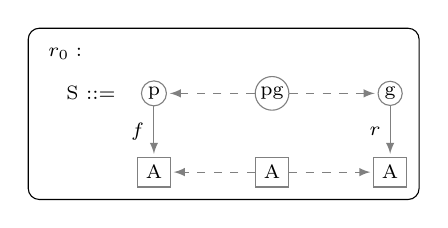
\begin{tikzpicture}[grammar]
	\node[rid] at (\ridX,\ridY) {$r_0:$};
	\draw (\lhsX,0) node[lhs] (lhs) {S ::=};
	
	\draw (0.5,0) node[t] (s1) {p};
	\draw (0.5,-1) node[nont] (s2) {A};
	\draw[edge] (s1) -- (s2) node [vledgeLabel] {$f$};
	%%
	\draw (2,0) node[t] (c1) {pg};
	\draw (2,-1) node[nont] (c2) {A};
	%%
	\draw (3.5,0) node[t] (t1) {g};
	\draw (3.5,-1) node[nont] (t2) {A};
	\draw[edge] (t1) -- (t2) node [vledgeLabel] {$r$};
	%%
	\draw[morph] (c1) -- (s1);
	\draw[morph] (c1) -- (t1);
	\draw[morph] (c2) -- (s2);
	\draw[morph] (c2) -- (t2);
	\end{tikzpicture}
	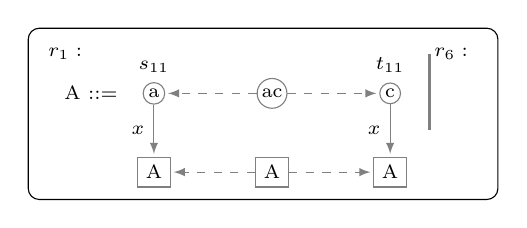
\begin{tikzpicture}[grammar]
	\node[rid] at (\ridX,\ridY) {$r_1:$};
	\draw (\lhsX,0) node[lhs] (lhs) {A ::=};
	
	\draw (0.5,0) node[t, label=90:$s_{11}$] (s1) {a};
	\draw (0.5,-1) node[nont] (s2) {A};
	\draw[edge] (s1) -- (s2) node [vledgeLabel] {$x$};
	%\draw node[uw] at (s1.east) (w-s1) {} [wedge] (s1) -- (w-s1);
	%%
	\draw (2,0) node[t] (c1) {ac};
	\draw (2,-1) node[nont] (c2) {A};
	%%
	\draw (3.5,0) node[t, label=90:$t_{11}$] (t1) {c};
	\draw (3.5,-1) node[nont] (t2) {A};
	\draw[edge] (t1) -- (t2) node [vledgeLabel] {$x$};
	%\draw node[uw] at (t1.north) (w-t1) {} [wedge] (t1) -- (w-t1);
	%%
	\draw[morph] (c1) -- (s1);
	\draw[morph] (c1) -- (t1);
	\draw[morph] (c2) -- (s2);
	\draw[morph] (c2) -- (t2);
	
	%%%%
	\draw[pipe] (4,\pipeBY) -- (4,\pipeUY);
	
	\node[rid] at (4.6,\ridY) {$r_6:$};
	\draw (4.6,0) node[empty] (s3) {$\emptyGraph$};
	\end{tikzpicture}
	
	\noindent
	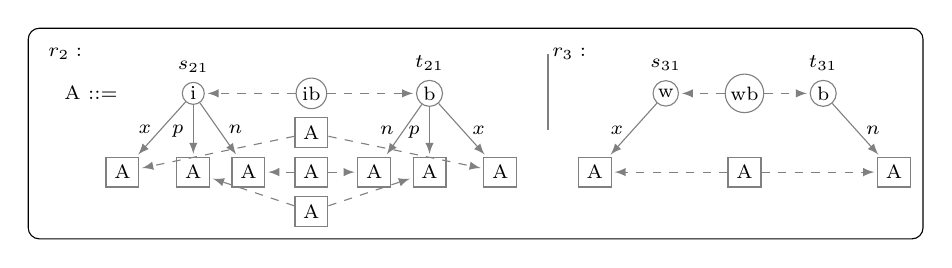
\begin{tikzpicture}[grammar]
	\node[rid] at (\ridX,\ridY) {$r_2:$};
	\draw (\lhsX,0) node[lhs] (lhs) {A ::=};
	
	\draw (1,0) node[t, label=90:$s_{21}$] (s1) {i};
	\draw (0.1,-1) node[nont] (s2) {A};
	\draw (1,-1) node[nont] (s3) {A};
	\draw (1.7,-1) node[nont] (s4) {A};
	\draw[edge] (s1) -- (s2) node [vledgeLabel] {$x$};
	\draw[edge] (s1) -- (s3) node [vledgeLabel] {$p$};
	\draw[edge] (s1) -- (s4) node [vredgeLabel] {$n$};
	%\draw node[uw] at (s1.north) (w-s1) {} [wedge] (s1) -- (w-s1);
	%%
	\draw (2.5,0) node[t] (c1) {ib};
	\draw (2.5,-0.5) node[nont] (c2) {A};
	\draw (2.5,-1) node[nont] (c4) {A};
	\draw (2.5,-1.5) node[nont] (c3) {A};
	%%
	\draw (4,0) node[t, label=90:$t_{21}$] (t1) {b};
	\draw (3.3,-1) node[nont] (t4) {A};
	\draw (4,-1) node[nont] (t3) {A};
	\draw (4.9,-1) node[nont] (t2) {A};
	\draw[edge] (t1) -- (t4) node [vledgeLabel] {$n$};
	\draw[edge] (t1) -- (t3) node [vledgeLabel] {$p$};
	\draw[edge] (t1) -- (t2) node [vredgeLabel] {$x$};
	%\draw node[uw] at (t1.north) (w-t1) {} [wedge] (t1) -- (w-t1);
	%%
	\draw[morph] (c1) -- (s1);
	\draw[morph] (c1) -- (t1);
	\draw[morph] (c2) -- (s2);
	\draw[morph] (c2) -- (t2);
	\draw[morph] (c3) -- (s3);
	\draw[morph] (c3) -- (t3);
	\draw[morph] (c4) -- (s4);
	\draw[morph] (c4) -- (t4);
	
	%%%%
	\draw[pipe] (5.5,\pipeBY) -- (5.5,\pipeUY);
	
	\node[rid] at (6.1,\ridY) {$r_3:$};
	
	\draw (7,0) node[t, label=90:$s_{31}$] (s5) {w};
	\draw (6.1,-1) node[nont] (s6) {A};
	\draw[edge] (s5) -- (s6) node [vledgeLabel] {$x$};
	%\draw node[uw] at (s5.north) (w-s5) {} [wedge] (s5) -- (w-s5);
	%%
	\draw (8,0) node[t] (c5) {wb};
	\draw (8,-1) node[nont] (c6) {A};
	%%
	\draw (9,0) node[t, label=90:$t_{31}$] (t5) {b};
	\draw (9.9,-1) node[nont] (t6) {A};
	\draw[edge] (t5) -- (t6) node [vredgeLabel] {$n$};
	%\draw node[uw] at (t5.north) (w-t5) {} [wedge] (t5) -- (w-t5);
	%%
	\draw[morph] (c5) -- (s5);
	\draw[morph] (c5) -- (t5);
	\draw[morph] (c6) -- (s6);
	\draw[morph] (c6) -- (t6);
	\end{tikzpicture}
	
	\noindent
	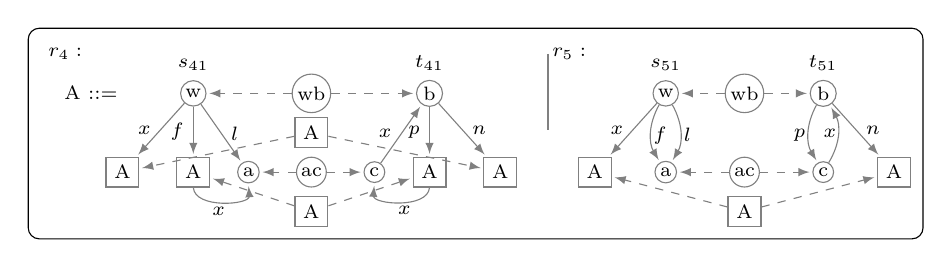
\begin{tikzpicture}[grammar]
	\node[rid] at (\ridX,\ridY) {$r_4:$};
	\draw (\lhsX,0) node[lhs] (lhs) {A ::=};
	
	\draw (1,0) node[t, label=90:$s_{41}$] (s1) {w};
	\draw (0.1,-1) node[nont] (s2) {A};
	\draw (1,-1) node[nont] (s3) {A};
	\draw (1.7,-1) node[t] (s4) {a};
	
	\draw[edge] (s1) -- (s2) node [vledgeLabel] {$x$};
	\draw[edge] (s1) -- (s3) node [vledgeLabel] {$f$};
	\draw[edge] (s3) to [bend right=90] (s4) node [below=10pt, left=5pt] {$x$};
	\draw[edge] (s1) -- (s4) node [vredgeLabel] {$l$};
	%\draw node[uw] at (s1.north) (w-s1) {} [wedge] (s1) -- (w-s1);
	%%
	\draw (2.5,0) node[t] (c1) {wb};
	\draw (2.5,-0.5) node[nont] (c2) {A};
	\draw (2.5,-1) node[t] (c4) {ac};
	\draw (2.5,-1.5) node[nont] (c3) {A};
	%%
	\draw (4,0) node[t, label=90:$t_{41}$] (t1) {b};
	\draw (3.3,-1) node[t] (t4) {c};
	\draw (4,-1) node[nont] (t3) {A};
	\draw (4.9,-1) node[nont] (t2) {A};
	\draw[edge] (t1) -- (t2) node [vredgeLabel] {$n$};
	\draw[edge] (t1) -- (t3) node [vledgeLabel] {$p$};
	\draw[edge] (t3) to [bend left=90] (t4) node [below=10pt, right=5pt] {$x$};
	\draw[edge] (t4) -- (t1) node [vledgeLabel] {$x$};
	%\draw node[uw] at (t1.north) (w-t1) {} [wedge] (t1) -- (w-t1);
	%%
	\draw[morph] (c1) -- (s1);
	\draw[morph] (c1) -- (t1);
	\draw[morph] (c2) -- (s2);
	\draw[morph] (c2) -- (t2);
	\draw[morph] (c3) -- (s3);
	\draw[morph] (c3) -- (t3);
	\draw[morph] (c4) -- (s4);
	\draw[morph] (c4) -- (t4);
	
	%%%%
	\draw[pipe] (5.5,\pipeBY) -- (5.5,\pipeUY);
	
	\node[rid] at (6.1,\ridY) {$r_5:$};
	
	\draw (7,0) node[t, label=90:$s_{51}$] (s5) {w};
	\draw (6.1,-1) node[nont] (s6) {A};
	\draw (7,-1) node[t] (s7) {a};
	\draw[edge] (s5) -- (s6) node [vledgeLabel] {$x$};
	\draw[edge] (s5) to [bend right] (s7) node [vbedgeLabel] {$f$};
	\draw[edge] (s5) to [bend left] (s7) node [above=10pt, right=1pt] {$l$};
	%\draw node[uw] at (s5.north) (w-s5) {} [wedge] (s5) -- (w-s5);
	%%
	\draw (8,0) node[t] (c5) {wb};
	\draw (8,-1.5) node[nont] (c6) {A};
	\draw (8,-1) node[t] (c7) {ac};
	%%
	\draw (9,0) node[t, label=90:$t_{51}$] (t5) {b};
	\draw (9,-1) node[t] (t7) {c};
	\draw (9.9,-1) node[nont] (t6) {A};
	\draw[edge] (t5) -- (t6) node [vredgeLabel] {$n$};
	\draw[edge] (t5) to [bend right] (t7) node [above=10pt, left=1pt] {$p$};
	\draw[edge] (t7) to [bend right] (t5) node [below=5pt] {$x$};
	%\draw node[uw] at (t5.north) (w-t5) {} [wedge] (t5) -- (w-t5);
	%%
	\draw[morph] (c5) -- (s5);
	\draw[morph] (c5) -- (t5);
	\draw[morph] (c6) -- (s6);
	\draw[morph] (c6) -- (t6);
	\draw[morph] (c7) -- (s7);
	\draw[morph] (c7) -- (t7);
	\end{tikzpicture}
	
	\noindent
	with $\sigma_0 = \emptyset$, $\sigma_1(s_{11}) = \sigma_2(s_{21}) = \sigma_3(s_{31}) = \sigma_4(s_{41}) =\sigma_5(s_{51}) = \{ (f,p), (x,a), $ $(x,i), (x,w), (p,i), (n,i), (l,w), (f,w) \}$ and $\tau_1(t_{11}) = \tau_2(t_{21}) = \tau_3(t_{31}) = \tau_4(t_{41}) $ $= \tau_5(t_{51}) = \{ (r,g), (x,c), (x,b), (p,b), (n,b)\}$ being the complete definition of the source and target embedding functions of the rules $r_0$ to $r_5$, respectively.
	
	The rule $r_0$ relates programs to graphs, $r_1$ actions to commands, $r_2$ ifs to branches, $r_3$ empty whiles to simple branches, $r_4$ filled whiles to filled loops with branches, $r_5$ whiles with one action to loops with branches with one command and, finally, $r_6$ produces an empty graph from a symbol $A$, what allows any derivation in the grammar to finish.
	
	The aforementioned triple graph $TG$ is in $L(TGG)$, because the derivation
	$
	\startTG{TGG} \tderiv{r_0}{}{} G_1 \tderiv{r_2}{}{} G_2 \tderiv{r_6}{}{} G_3 \tderiv{r_1}{}{} G_4 \tderiv{r_6}{}{} G_5 \tderiv{r_1}{}{} G_6 \tderiv{r_4}{}{} G_7 \tderiv{r_1}{}{} G_8 \tderiv{r_6}{}{} G_9 \tderiv{r_1}{}{} G_{10} \tderiv{r_6}{}{} TG
	$
	is a derivation in TGG with appropriate $G_i$ for $1 \le i \le 10$.
\end{example}

Ultimately, consider the definitions of $\Gamma\text{-boundary}$ graphs and BNCE TGG, that are necessary for the next section.

\begin{definition}
	A $\Gamma\text{-boundary}$ graph $G$ is such that vertices labeled with any symbol from $\Gamma$ are not neighbors. That is, the graph $G$ is $\Gamma\text{-boundary}$ if, and only if, there is no $(v,l,w) \in E_G$ with $\phi_G(v) \in \Gamma$ and $\phi_G(w) \in \Gamma$.
\end{definition}

\begin{definition}
	\label{def:bncetgg}
	A boundary triple graph grammar with neighborhood-controlled embedding (BNCE TGG) is such that non-terminal vertices of the right-hand sides of rules are not neighbors. That is, the NCE triple graph grammar $TGG$ is boundary if, and only if, for all its rules' right-hand sides $R_s \ms{} R_c \mt{} R_t$, $R_s$, $R_c$, and $R_t$ are $\Gamma\text{-boundary}$ graphs.
\end{definition}

\section{Model Transformation with NCE TGG}
\label{sec:modeltrans}
As already introduced, TGG can be used to characterize languages of triple graphs holding correctly transformed models. That is, one can interpret a TGG as the description of the correctly-transformed relation between two sets of models $\mathcal{S}$ and $\mathcal{T}$, where two models $G \in \mathcal{S}$ and $T \in \mathcal{T}$ are in the relation if, and only if, $G$ and $T$ are respectively, source and target graphs of any triple graph of the language $L(TGG)$. That being said, we are interested in this section on defining a model transformation algorithm that interprets a NCE TGG $TGG$ to transform a source model $G$ into one of its correspondent target models $T$ according to the correctly-transformed relation defined by $TGG$.

For that end, let $TGG = (\Sigma = \Sigma_s \cup \Sigma_t, \Delta, S, P)$ be a triple graph grammar defining the correctly-transformed relation between two arbitrary sets of graphs $\mathcal{S}$ over $\Sigma_s$ and $\mathcal{T}$ over $\Sigma_t$. And let $G \in \mathcal{S}$ be a source graph. We want to find a target graph $T \in \mathcal{T}$ such that $G \ms{} C \mt{} T \in L(TGG)$. To put in words, we wish to find a triple graph holding $G$ and $T$ that is in the language of all correctly transformed models. Hence, the model transformation problem is reduced--- according to the definition of triple graph language (see Definition \ref{def:tlanguage})--- to the problem of finding a derivation $\startTG{TGG} \tderivtr{TGG} G \ms{} C \mt{} T$.

Our strategy to solve this problem is, first, to get a derivation for $G$ with the source part of $TGG$ and, then, construct the derivation $\startTG{TGG} \tderivtr{TGG} G \ms{} C \mt{} T$. For this purpose, consider the definition of the $\source$ function, that extracts the source part of a production rule.

\begin{definition}
	\label{def:source}
	Let $r = (A \pro (G_s \ms{} G_c \mt{} G_t), \omega_s, \omega_t)$ be a production rule of a triple graph grammar, $\source(r) = (A \pro G_s,\omega_s)$ gives the source part of $r$. Moreover, $\source^{-1}((A \pro G_s,\omega_s)) = r$ gives the original rule of a source rule.
\end{definition}

\begin{definition}
	\label{def:Source}
	Let $TGG = (\Sigma, \Delta, S, P)$ be a triple graph grammar, $\Source(TGG) = (\Sigma, \Delta, S, \source(P))$ gives the source grammar of $TGG$.
\end{definition}

Furthermore, consider the definition of the non-terminal consistent (NTC) property for TGG, which assures, that non-terminal vertices of the correspondent graphs are connected to vertices with the same label in the source and target graphs.

\begin{definition}
	A triple graph grammar $TGG = (\Sigma, \Delta, S, P)$ is non-terminal consistent (NTC) if and only if, for all rules $(A \pro (G_s \ms{ms} G_c \mt{mt} G_t), \omega_s, \omega_t) \in P$, the following holds:
	\begin{enumerate}
		\item $\forall c \in V_{G_c} \. \text{if } \phi_{G_c}(c) \in \Gamma \text{ then } \phi_{G_c}(c) = \phi_{G_s}(ms(c)) = \phi_{G_t}(mt(c))$ and
		\item For the sets $N_s = \{v \st \phi_{G_s}(v) \in \Gamma\}$ and $N_t = \{v \st \phi_{G_t}(v) \in \Gamma\}$, the range-restricted functions $(ms \rrestr N_s)$ and $(mt \rrestr N_t)$ are bijective.
	\end{enumerate}
\end{definition}

Finally, the following result gives us an equivalence between a derivation in $TGG$ and a derivation in its source grammar $S(TGG)$, which allows us to construct our goal derivation of $G \ms{} C \mt{} T$ in $TGG$ using the derivation of $G$ in $S(TGG)$.

\begin{theorem}
	\label{thm:one_d_enough}
	Let $TGG = (\Sigma, \Delta, S, P)$ be a NTC TGG and $k \ge 1$, \\
	$D = \startTG{TGG} \tderiv{r_0}{s_0,c_0,t_0}{} G^1 \tderiv{r_1}{s_1,c_1,t_1}{} \dots \tderiv{r_{k-1}}{s_{k-1},c_{k-1},t_{k-1}}{} G^k$ is a derivation in $TGG$ if, and only if, $\overline{D} = \startG{S(TGG)} \deriv{s(r_0)}{s_0}{} G^1_s \deriv{s(r_1)}{s_1}{} \dots \deriv{s(r_{k-1})}{s_{k-1}}{} G^k_s$ is a derivation in $S(TGG)$.
\end{theorem}
\begin{proof}
	We want to show that if $D$ is a derivation in $TGG = (\Sigma, \Delta, S, P)$, then $\overline{D}$ is a derivation in $SG := S(TGG) = (\Sigma, \Delta, S, SP)$, and vice-versa. We prove it by induction in the following.
	
	First, for the induction base, since, $\startTG{TGG} \tderiv{r_0}{s_0,c_0,t_0}{TGG} G^1$, then expanding $\startTG{TGG}$ and $G^1$, we have
	\begin{align*}
		& Z_s \ms{} Z_c \mt{} Z_t \tderiv{r_0}{s_0,c_0,t_0}{TGG} G^1_s \ms{} G^1_c \mt{} G^1_t \text{, then, by Definition \ref{def:tgg_dstep},}\\
		& r_0 = (S \pro (R_s \ms{} R_c \mt{} R_t), \omega_s, \omega_t) \in P \text{ and, by Definition \ref{def:source},}\\
		& \source(r_0) = (S \pro R_s, \omega_s) \in SP
	\end{align*}
	
	Hence, using it plus the configuration of $\phi_{Z_s}(s_0)$, $V_{G^1_s}$, $E_{G^1_s}$ and $\phi_{G^1_s}$ and the equality $Z_s = \startG{SG}$, we have, by Definition \ref{def:gg_dstep}, $\startG{SG} \deriv{\source(r_0)}{s_0}{SG} G^1_s$.
	
	In the other direction, we choose $c_0, t_0$ from the definition of $\startTG{TGG}$, with $\phi_{Z_c}(c_0) = S$ and  $\phi_{Z_t}(t_0) = S$. In this case, since,
	\begin{align*}
		& \startG{SG} \deriv{s(r_0)}{s_0}{SG} G^1_s \text{, then by Definition \ref{def:gg_dstep},}\\
		& \source(r_0) = (S \pro R_s, \omega_s) \in SP \text{ and, using the bijectivity of $\source$, we get}\\
		& r_0 = \source^{-1}(s(r_0)) = (S \pro (R_s \ms{} R_c \mt{} R_t), \omega_s, \omega_t) \in P
	\end{align*}
	
	Hence, using it plus the configuration of $\phi_{\startG{SG}}(s_0)$, $V_{G^1_s}$, $E_{G^1_s}$ and $\phi_{G^1_s}$, the equality $Z_s = \startG{SG}$ and constructing $V_{G^1_c}$, $V_{G^1_t}$, $E_{G^1_c}$, $E_{G^1_t}$, $\phi_{G^1_c}$, $\phi_{G^1_t}$ from $Z_c$ and $Z_t$ according to the Definition \ref{def:tgg_dstep} $\startTG{TGG} \tderiv{r_0}{s_0,c_0,t_0}{TGG} G^1_s \ms{} G^1_c \mt{} G^1_t$.
	
	Now, for the induction step, we want to show that if $\startTG{TGG} \tderivtr{TGG} G^i$ $\tderiv{r_{i}}{s_{i},c_{i},t_{i}}{TGG} G^{i+1}$ is a derivation in $TGG$, then $\startG{SG} \derivtr{SG} G^i_s \deriv{s(r_{i})}{s_{i}}{SG} G^{i+1}_s$ is a derivation in $SG$ and vice-versa, provided that the equivalence holds for the first $i$ steps, so we just have to show it for the step $i+1$.
	
	So, since, $G^i \tderiv{r_{i}}{s_{i},c_{i},t_{i}}{TGG} G^{i+1}$, that is
	\begin{align*}
		& G^i_s \ms{ms_i} G^i_c \mt{mt_i} G^i_t \tderiv{r_i}{s_i,c_i,t_i}{TGG} G^{i+1}_s \ms{} G^{i+1}_c \mt{} G^{i+1}_t \text{, then, by Definition \ref{def:tgg_dstep},}\\
		& r_i = (S \pro (R_s \ms{} R_c \mt{} R_t), \omega_s, \omega_t) \in P \text{, and by Definition \ref{def:source},}\\
		& \source(r_i) = (S \pro R_s, \omega_s) \in SP
	\end{align*}
	
	Hence, using it plus the configuration of $\phi_{G^i_s}(s_i)$, $V_{G^{i+1}_s}$, $E_{G^{i+1}_s}$ and $\phi_{G^{i+1}_s}$, we have, by Definition \ref{def:gg_dstep}, $G_s^i \deriv{\source(r_i)}{s_i}{SG} G^{i+1}_s$.
	
	In the other direction, we choose, using the bijectivity from the range restricted function $\source$, stemming from the NTC property, $c_i = ms_i^{-1}(s_i), t_i = mt_i(c_i)$. Moreover, since $TGG$ is NTC, and because, by induction hypothesis, $\startTG{TGG} \tderivtr{TGG} G^i$ is a derivation in $TGG$ and $\phi_{G^i_s}(s_i) \in \Gamma$, it is clear that $\phi_{G^i_s}(s_i) = \phi_{G^i_c}(c_i) = \phi_{G^i_t}(t_i)$.
	
	In this case, since
	\begin{align*}
		& G^{i}_s \deriv{s(r_i)}{s_i}{SG} G^{i+1}_s \text{, then, by Definition \ref{def:gg_dstep},}\\
		& \source(r_i) = (A \pro R_s, \omega_s) \in SP \text{ and, using the bijectivity of $\source$, we get }\\
		& r_i = \source^{-1}(s(r_i)) = (A \pro (R_s \ms{} R_c \mt{} R_t), \omega_s, \omega_t) \in P
	\end{align*} 
	
	Hence, using, additionally, the configuration of $\phi_{G^i_s}(s_i)$, $\phi_{G^i_c}(c_i)$, $\phi_{G^i_t}(t_i)$, $V_{G^{i+1}_s}$, $E_{G^{i+1}_s}$ and $\phi_{G^{i+1}_s}$ and constructing $V_{G^{i+1}_c}$, $V_{G^{i+1}_t}$, $E_{G^{i+1}_c}$, $E_{G^{i+1}_t}$, $\phi_{G^{i+1}_c}$, $\phi_{G^{i+1}_t}$ from $G^i_c$ and $G^i_t$ according to the Definition \ref{def:tgg_dstep}, we have 
	\begin{equation*}
		G^i_s \ms{} G^i_c \mt{} G^i_t \tderiv{r_i}{s_i,c_i,t_i}{TGG} G^{i+1}_s \ms{} G^{i+1}_c \mt{} G^{i+1}_t
	\end{equation*}
	
	This finishes the proof.\qed
\end{proof}

Therefore, the problem of finding a derivation $D = \startTG{TGG} \tderivtr{} G \ms{} C \mt{} T$ in $TGG$ is reduced to finding a derivation $\overline{D} = \startG{S(TGG)} \derivtr{} G$ in $S(TGG)$, what can be done with the procedure in \cite{rozenberg1986boundary}. The final construction of the triple graph $G \ms{} C \mt{} T$ becomes then just a matter of creating $D$ out of $\overline{D}$.

The complete transformation procedure is presented in the Algorithm \ref{alg:transform}. Thereby, it is required that the TGG be a BNCE TGG (see Definition \ref{def:bncetgg}) and be neighborhood preserving (NP) \cite{rozenberg1986boundary,skodinis1998neighborhood}, what poses no problem to our procedure, since any BNCE graph grammar can be transformed into the neighborhood preserving normal form. 
\begin{algorithm}[h]
	\caption{Transformation Algorithm for NP NTC BNCE TGG}
	\begin{algorithmic}[h]
		\Require $TGG \text{ is a valid NP NTC BNCE triple graph grammar}$
		\Require $G \text{ is a valid graph over } \Sigma$
		\Function{$transform$}{$TGG=(\Sigma, \Delta, S, P), G=(V_G,E_G,\phi_G)$}{$:Graph$}
		\State $SG \gets S(TGG)$ \Comment{see Definition \ref{def:source}}
		\State $\overline{D} \gets parse(SG,G)$ \Comment{use procedure in \cite{rozenberg1986boundary}}
		\If{$\overline{D} = \startG{SG} \derivtr{SG} G$} \Comment{if parsed successfully}
		\State From $\overline{D}$, construct $D = \startTG{TGG} \tderivtr{TGG} G \ms{} C \mt{} T$  \Comment{see Theorem \ref{thm:one_d_enough}}
		\State \Return {$\Just T$}
		\Else
		\State \Return {$\Nothing$} \Comment{no $T$ satisfies $(G \ms{} C \mt{} T) \in L(TGG)$}
		\EndIf
		\EndFunction 
		\Ensure $return \text{ is either } \Nothing \text{ or } \Just T \text{, such that } (G \ms{} C \mt{} T) \in L(TGG)$
	\end{algorithmic}
	\label{alg:transform}
\end{algorithm}

\section{Evaluation}
\label{sec:eval}
In order to evaluate the usability of the proposed BNCE TGG formalism, we compare the number of rules and elements (vertices, edges, and mappings) we needed to describe some model transformations in BNCE TGG and in standard TGG without application conditions. Table \ref{tab:formalism-eval} presents these results.

In the case of $Pseudocode2Controlflow$, our proposed approach shows a clear advantage against the standard TGG formalism. We judge that similarly to what happens to programming languages, this advantage stems from the very nested structure of $Pseudocode$ and $Controlflow$ graphs. That is, for instance, in rule the $r_2$ of this TGG (see Example \ref{ex:pseudocode2controlflow}), a node in a positive branch of an $if$-labeled vertex is never connected with a node in the negative branch. This disjunctive aspect allows every branch to be defined in the rule (as well as effectively parsed) independently of the other branch. This characteristic makes it possible for BNCE TGG rules to be defined in a very straightforward manner and reduces the total number of elements necessary.

\begin{table}[t]
	\setlength{\tabcolsep}{10pt}
	\centering
	\begin{tabular}{l r r r r }
		\hline
		& \multicolumn{2}{c}{Standard TGG} & \multicolumn{2}{c}{BNCE TGG}\\
		Transformation 			& Rules & Elements 	& Rules & Elements\\
		\hline
		Pseudocode2Controlflow	& 45			& 1061	& \textbf{7}	& \textbf{185} \\
		BTree2XBTree			& \textbf{4}	& \textbf{50}	& 5		& 80 \\
		Star2Wheel				& -				& -		& \textbf{6} 	& \textbf{89} \\
		Class2Database			& \textbf{6}	& \textbf{98}	& -	& - \\
		\hline
	\end{tabular}
	\caption{Results of the usability evaluation of the BNCE TGG formalism in comparison with the standard TGG for the model transformation problem}
	\label{tab:formalism-eval}
\end{table}

In addition to that, the use of non-terminal symbols gives BNCE TGG the power to represent abstract concepts very easily. For example, whereas the rule $r_1$ encodes, using only few elements, that after each $action$ comes any statement $A$, which can be another $action$, an $if$, a $while$ or nothing (an empty graph), in the standard TGG without application condition or any special inheritance treatment, we need to write a different rule for each of these cases. For the whole grammar, we need to consider all combinations of $actions$, $ifs$ and $whiles$ in all rules, what causes the great number of rules and elements.

The $Star2Wheel$ transformation consists of transforming star graphs, which are complete bipartite graphs $K_{1,k}$--- where the partitions are named center and border--- to wheel graphs, that can be constructed from star graphs by adding edges between border vertices to form a minimal cycle. We could not describe this transformation in standard TGG, especially because of the rules' monotonicity (see Definition \ref{def:stgg}). That is, we missed the possibility to erase edges in a rule, feature that we do have in the semantics of BNCE TGG through the embedding mechanism.

The $Class2Database$ transformation consists of transforming class diagrams, similar to UML class diagrams, to database diagrams, similar to physical entity-relationship diagrams. We could not describe this transformation in BNCE TGG by the fact that the information about the production of a terminal vertex is owned exclusively by one derivation step. That is, this information cannot be used by other derivation steps (the BNCE grammar is context-free). Thus, in the case of $Class2Database$, in which an \textit{association} is connected to two \textit{classes}, each been produced by two different derivation steps, we could not connect one association with two classes.

\section{Conclusion}
\label{sec:conclusion}
We present in this paper a new triple graph grammar formalism, called NCE TGG, that is the result of mixing NCE graph grammars \cite{janssens1982graph} with TGG \cite{schurr1994specification} and that introduces for the first time, as far as we know, non-terminal symbols to TGG. Furthermore, we demonstrate how BNCE TGG can be used in the practice to solve the model transformation problem.

An experimental evaluation in Section \ref{sec:eval} assesses the usability of BNCE TGG in comparison with standard TGG and reveals that our proposed approach has potential. In special, we could express one transformation with BNCE TGG that we could not with TGG. And, from the other three evaluated transformations, BNCE TGG outperformed TGG in one use case with a much smaller grammar. In our view, smaller and less complex rules tend to be easier to comprehend and validate, what in turn makes formal specifications in BNCE TGG more suitable for safety-critical systems.

We are aware that this disadvantage for TGG comes from the absence of (negative and positive) application conditions, but we also argue that such mechanisms are often unhandy for tools and researchers that want to reason about it. In this sense, the use of non-terminal symbols seems to be a neater alternative to it.

As a future work, we intend to carry out a broader usability and performance evaluation of our approach and extend NCE graph grammars with an application condition mechanism that should allow it to express more languages than it can now. Finally, although the extension of our approach for the bidirectional transformation problem is straightforward, the same does not seem to be true for the model synchronization problem. Whereas the former consists of simply performing transformation from source to target and from target to source, the latter consists of transforming already generated models in both directions without creating them from scratch and using only the information of the modifications. Therefore, we are also interested in studying how our approach can be used to solve it.

%
% ---- Bibliography ----
%
% BibTeX users should specify bibliography style 'splncs04'.
% References will then be sorted and formatted in the correct style.
%
\bibliographystyle{splncs04}
\bibliography{bibliography}
\end{document}
